\ifdefined\standalone
\documentclass[12pt]{article}
\usepackage[a4paper, margin=1in]{geometry}
\usepackage[utf8]{inputenc}
\usepackage{textcomp}
\usepackage{amsmath}
\usepackage{graphicx}
\usepackage{float}
\usepackage[hidelinks]{hyperref}
\usepackage{tikz}
\usetikzlibrary{decorations.pathmorphing,patterns}
\begin{document}
\fi

\section{Insulated Multi-Layer Steel Plate}

This case considers steady-state one-dimensional heat conduction through a multilayer composite slab composed of a central steel layer of thickness $L_{\text{steel}} = 1~\mathrm{cm}$, symmetrically covered by two insulation layers of thickness $L_{\text{ins}} = 2~\mathrm{cm}$ each. The assembly is subjected to asymmetric convective boundary conditions: the hot-side surface is exposed to ambient air at $T_{\infty,t} = 480~^\circ\mathrm{C}$, while the cold-side surface is exposed to air at $T_{\infty,b} = 20~^\circ\mathrm{C}$. The slab is heated for a sufficiently long duration (10~hours) to ensure steady-state conditions. The convective heat transfer coefficient is assumed identical on both sides and equal to $h_c = 10~\mathrm{W\,m^{-2}\,K^{-1}}$ (see Fig.~\ref{fig:isp_fixed_configuration}). The thermophysical properties of the materials are summarized in Table~\ref{tab:thermal_properties_insulated_steel_plate}.

\begin{table}[H]
\centering
\caption{Thermophysical properties of the materials.}
\label{tab:thermal_properties_insulated_steel_plate}
\renewcommand{\arraystretch}{1.3}
\begin{tabular}{l c c c}
\hline
Material &
$k$ ($\mathrm{W\,m^{-1}\,K^{-1}}$) &
$c_p$ ($\mathrm{J\,kg^{-1}\,K^{-1}}$) &
$\rho$ ($\mathrm{kg\,m^{-3}}$) \\
\hline
Steel        & 50.0 & 500  & 7500 \\
Insulation  & 0.2  & 1000 & 200  \\
\hline
\end{tabular}
\end{table}

At steady state, the heat flux is constant through the slab and is given by \cite{incropera_fundamentals_2007}:
\begin{equation}
q'' =
\frac{T_{\infty,t} - T_{\infty,b}}{
\frac{1}{h_c}
+ \frac{L_{\text{ins}}}{k_{\text{ins}}}
+ \frac{L_{\text{steel}}}{k_{\text{steel}}}
+ \frac{L_{\text{ins}}}{k_{\text{ins}}}
+ \frac{1}{h_c}}
\end{equation}

The temperature field within each layer is piecewise linear between successive interfaces, and the temperatures at the interfaces are expressed as: 
\begin{equation}
\left\{
\begin{aligned}
T_0 &= T_{\infty,t} - \frac{q''}{h_c}
&& \text{: hot-side surface temperature}\\
T_1 &= T_0 - q'' \frac{L_{\text{ins}}}{k_{\text{ins}}}
&& \text{: interface between hot-side insulation and steel}\\
T_2 &= T_1 - q'' \frac{L_{\text{steel}}}{k_{\text{steel}}}
&& \text{: interface between steel and cold-side insulation}\\
T_3 &= T_2 - q'' \frac{L_{\text{ins}}}{k_{\text{ins}}}
&& \text{: cold-side surface temperature}
\end{aligned}
\right.
\end{equation}

\begin{figure}[H]
\centering

\begin{minipage}{0.48\textwidth}
    \centering
    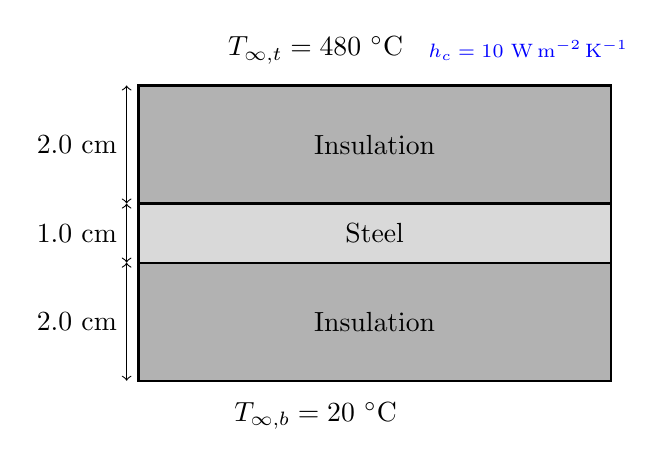
\begin{tikzpicture}[scale=0.75]

    % Steel
    \draw[fill=gray!30,thick] (0,0) rectangle (8,1);
    \node at (4,0.5) {Steel};

    % Bottom insulation (cold side)
    \draw[fill=gray!60,thick] (0,-2) rectangle (8,0);
    \node at (4,-1) {Insulation};
    \node[below] at (3,-2.2) {$T_{\infty,b} = 20~^\circ\mathrm{C}$};

    % Top insulation (hot side)
    \draw[fill=gray!60,thick] (0,1) rectangle (8,3);
    \node at (4,2) {Insulation};
    \node[above] at (3,3.2) {$T_{\infty,t} = 480~^\circ\mathrm{C}$};

    % Dimensions
    \draw[<->] (-0.2,0) -- (-0.2,1);
    \node[left] at (-0.2,0.5) {$1.0~\mathrm{cm}$};

    \draw[<->] (-0.2,-2) -- (-0.2,0);
    \node[left] at (-0.2,-1) {$2.0~\mathrm{cm}$};

    \draw[<->] (-0.2,1) -- (-0.2,3);
    \node[left] at (-0.2,2) {$2.0~\mathrm{cm}$};

    % Convection annotation
    \node[blue] at (6.6,3.6) {\scriptsize $h_c = 10~\mathrm{W\,m^{-2}\,K^{-1}}$};

    \end{tikzpicture}
    \caption{Schematic of the insulated steel plate configuration.}
    \label{fig:isp_fixed_configuration}
\end{minipage}
\hfill
\begin{minipage}{0.48\textwidth}
    \centering
    \includegraphics[width=\textwidth]{insulated_steel_plate.png}
    \caption{Temperature profile as a function of depth within the multilayer slab.}
    \label{fig:temperature_profile}
\end{minipage}

\end{figure}

\ifdefined\standalone
\end{document}
\fi

